\section{The block bound}\label{sec:blocks}

We prove that every rule for choosing the order of visits within a block gives an upper bound for $\beta$ (\cref{thm:block}).

\subsection{The constant in terms of a Poisson process}

For a finite set $A\subset\R^2$ let $L(A)$ be the length of a shortest closed tour through the points of $A$, with $L(A)=0$ if $A$ has fewer than two points. In this notation the $L_n$ of \cref{sec:intro} is $L(\{X_1,\dots,X_n\})$. We use the following standard consequence of the theorem of Beardwood, Halton and Hammersley \cite{BeardwoodHaltonHammersley1959,Steele1997}. It is stated in this form in \cite[equation~(5)]{DongCao2026}; the short proof follows the sketch in \cite[Section~2.1]{Steinerberger2015}, attributed there to Steele.

\begin{lem}\label{lem:poisson}
Let $\Pi$ be a Poisson process of intensity $1$ in the plane, and let $\Lambda_W=[0,W]^2$. Then
\[
\lim_{W\to\infty}\frac{\E\,L(\Pi\cap \Lambda_W)}{W^2}=\beta .
\]
\end{lem}

\begin{proof}
Put $\ell_n=\E\,L_n$. By a theorem of Few \cite{Few1955}, any $n\ge1$ points of the unit square lie on a path of length at most $\sqrt{2n}+1.75$. Closing the path adds at most $\sqrt2$, so $L(A)\le c\sqrt n$ with $c=2\sqrt2+1.75$ for every set $A$ of $n\ge1$ points in the unit square, and $\ell_n/\sqrt n\to\beta$ by bounded convergence. Hence for every $\eps>0$ there is a constant $C_\eps$ with $|\ell_n-\beta\sqrt n|\le\eps\sqrt n+C_\eps$ for all $n\ge0$.

Let $N$ be the number of points of $\Pi$ in $\Lambda_W$. It has the Poisson distribution with mean $W^2$, and given $N=n$ the points are independent and uniform in $\Lambda_W$. Scaling by $W$ gives $\E\,L(\Pi\cap \Lambda_W)=W\,\E\,\ell_N$, and therefore
\[
\bigl|\E\,L(\Pi\cap \Lambda_W)-\beta W\,\E\sqrt N\bigr|\le \eps W\,\E\sqrt N+C_\eps W .
\]
By Jensen's inequality, $\E\sqrt N\le W$. In the other direction, $\sqrt N-W=(N-W^2)/(\sqrt N+W)\ge-|N-W^2|/W$ and $\E|N-W^2|\le(\operatorname{Var}N)^{1/2}=W$, so $\E\sqrt N\ge W-1$. Dividing by $W^2$ and letting $W\to\infty$ and then $\eps\to0$ gives the claim.
\end{proof}

\subsection{Blocks, orders and rules}

Fix an integer $k\ge1$ and a real number $h>0$. Let $Z_1,\dots,Z_k$ be exponential random variables with mean $1$ and let $U_0,\dots,U_k$ be uniform on $[0,1]$, all independent. Put
\[
P_i=\bigl(Z_1+\dots+Z_i,\;h^2U_i\bigr),\qquad 0\le i\le k .
\]
We call $(P_0,\dots,P_k)$ a \emph{block}, the $Z_i$ its \emph{gaps} and the $U_i$ its \emph{heights}; the height of a point is its second coordinate divided by $h^2$. A block is a copy, magnified by the factor $h$, of $k+1$ consecutive points of a Poisson process of intensity $1$ in a horizontal strip of height $h$: there the horizontal distances between consecutive points are exponential with mean $1/h$ and the vertical coordinates are uniform on an interval of length $h$. The proof of \cref{thm:block} makes this precise.

An \emph{order} is a permutation $\pi$ of $\{1,\dots,k-1\}$. It stands for the path that starts at $P_0$, visits the \emph{interior points} $P_1,\dots,P_{k-1}$ in the order $P_{\pi(1)},\dots,P_{\pi(k-1)}$, and ends at $P_k$; we write $L_\pi$ for the length of this path. A \emph{rule} is a measurable map $\rho$ from $[0,\infty)^k\times[0,1]^{k+1}$ to the set of orders. It chooses an order from the gaps and heights of the block, and we write $L_\rho$ for the length of the path it chooses (\cref{fig:strip}).

\begin{figure}[ht]
\centering
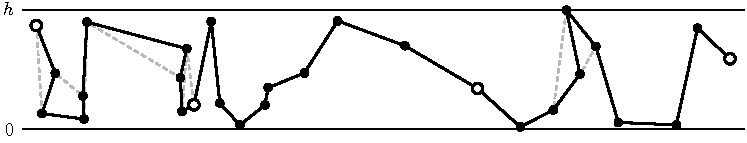
\includegraphics[width=\textwidth]{fig_strip}
\caption{Three consecutive blocks of a strip for $k=\MainK$ and $h=\MainH$, drawn from a simulation. Open circles mark the first and the last point of each block. The solid line is the path chosen by the rule of \cref{sec:computation} for \cref{thm:main}; where it differs from the order of the first coordinates, that order is shown by a dashed line.}
\label{fig:strip}
\end{figure}

\begin{thm}[Block bound]\label{thm:block}
For every integer $k\ge1$, every $h>0$ and every rule $\rho$,
\[
\beta\le\frac{\E\,L_\rho}{kh}.
\]
\end{thm}

We call $\E\,L_\rho/(kh)$ the \emph{value} of the rule $\rho$. For $k=1$ there is one order, and the value is the expected distance between consecutive points of a strip; this is the bound of \cite{BeardwoodHaltonHammersley1959}, where $h=\sqrt3$. For the rule that chooses a shortest path (the first one in a fixed list of the orders, if there are several), the theorem is the bound \eqref{eq:tuple} stated in \cite[Section~3.1]{YuCarlsson2023}; we call the value of this rule the \emph{shortest-path value} for $k$ and $h$, and no rule has a smaller value.

The computation of \cite{YuCarlsson2023} already uses a rule of another kind, which chooses one order on each part of a partition; this order need not be shortest at every point of the part. For arbitrary rules and $k=5$ the theorem is Theorem~4 of \cite{DongCao2026}, and the proof below follows the proof given there, with $5$ replaced by $k$ and the strips joined in a slightly different way.

\begin{proof}
Every path in a block has length at most $k(Z_1+\dots+Z_k+h^2)$, so $\E\,L_\rho<\infty$.

Let $\Pi$ be a Poisson process of intensity $1$ in the plane, let $q\ge1$ be an integer and $W=qh$. For $1\le j\le q$ let $S_j=[0,\infty)\times[(j-1)h,jh)$. Almost surely no point of $\Pi$ has second coordinate $W$, and the points of $\Pi$ in $S_j$ have distinct first coordinates; let $P^j_1,P^j_2,\dots$ be these points in increasing order of the first coordinate. Add an auxiliary point $P^j_0$ with first coordinate $0$ and second coordinate $(j-1)h+Y^j_0$, where $Y^j_0$ is uniform on $[0,h)$ and independent of everything else. For $i\ge1$ let $\Delta^j_i$ be the first coordinate of $P^j_i$ minus that of $P^j_{i-1}$, and let $(j-1)h+Y^j_i$ be the second coordinate of $P^j_i$. Then the $\Delta^j_i$, $i\ge1$, are independent and exponential with mean $1/h$, the $Y^j_i$, $i\ge0$, are independent and uniform on $[0,h)$, and the two families are independent of each other: the first coordinates of the points in $S_j$ form a Poisson process of intensity $h$ on $[0,\infty)$, and the second coordinates are independent marks \cite{Kingman1993}.

For $b\ge0$, the points $P^j_{kb},P^j_{kb+1},\dots,P^j_{k(b+1)}$ form the $b$th block of the strip. Translating them so that $P^j_{kb}$ has first coordinate $0$ and the lower edge of the strip has second coordinate $0$, and then multiplying by $h$, gives $k+1$ points with the distribution of a block: the gaps are $h\Delta^j_{kb+1},\dots,h\Delta^j_{kb+k}$ and the heights are $Y^j_{kb}/h,\dots,Y^j_{kb+k}/h$. Let the rule $\rho$ choose an order for it, and let $C^j_b$ be the length of the corresponding path from $P^j_{kb}$ to $P^j_{k(b+1)}$ in the strip. Then $C^j_b$ has the distribution of $L_\rho/h$.

Let $K_j$ be the number of points of $\Pi$ in $S_j\cap \Lambda_W$ and $B_j=1+\lfloor K_j/k\rfloor$. The paths of the blocks $0,1,\dots,B_j-1$ share endpoints and join to a walk $\Gamma_j$ from $P^j_0$ to $P^j_{kB_j}$, whose length we denote by $|\Gamma_j|$. Since $kB_j>K_j$, this walk visits every point of $\Pi$ in $S_j\cap \Lambda_W$.

The $b$th block is used, that is $b<B_j$, exactly when $kb\le K_j$. For $b=0$ this always holds. For $b\ge1$ it is the event $\Delta^j_1+\dots+\Delta^j_{kb}\le W$, which is determined by $\Delta^j_1,\dots,\Delta^j_{kb}$. The length $C^j_b$ is a function of $\Delta^j_{kb+1},\dots,\Delta^j_{kb+k}$ and $Y^j_{kb},\dots,Y^j_{kb+k}$, so it is independent of this event; this is the argument of Wald's identity. (The last block that is used contains the gap across the line $x=W$, which tends to be longer than a typical gap. This does not matter: each term of the sum below belongs to a fixed $b$, and none is conditioned on $b$ being the last index used. Nor need the lengths $C^j_b$ for different $b$ be independent; they are not, since consecutive blocks share a point.) Since all terms are non-negative,
\begin{equation}\label{eq:strip}
\E\,|\Gamma_j|=\sum_{b\ge0}\E\bigl[C^j_b\,;\,b<B_j\bigr]=\sum_{b\ge0}\Pr(b<B_j)\,\E\,C^j_b=\E B_j\cdot\frac{\E\,L_\rho}{h}\le\Bigl(1+\frac{hW}{k}\Bigr)\frac{\E\,L_\rho}{h},
\end{equation}
because $\E K_j=hW$.

The endpoint $P^j_{kB_j}$ of $\Gamma_j$ has first coordinate $W+R_j$ with $R_j>0$. Since $K_j<kB_j\le K_j+k$, it is one of the first $k$ points of $\Pi$ in $S_j$ to the right of $\Lambda_W$, and the $k$th of these has first coordinate $W+G_j$, where $G_j$ is a sum of $k$ independent exponential variables with mean $1/h$. Hence $R_j\le G_j$ and $\E\,R_j\le k/h$.

Now traverse $\Gamma_1$ from $P^1_0$ to its endpoint, go straight to the endpoint of $\Gamma_2$, traverse $\Gamma_2$ backwards to $P^2_0$, go straight to $P^3_0$, and so on through all $q$ strips; finally return straight to $P^1_0$. The endpoints of $\Gamma_j$ and $\Gamma_{j+1}$ are at distance at most $2h+R_j+R_{j+1}$, and two auxiliary points in adjacent strips are at distance at most $2h$. Each $R_j$ occurs in at most one of these segments between adjacent strips. The final segment starts at the endpoint of $\Gamma_q$ if $q$ is odd and at $P^q_0$ if $q$ is even, and in both cases its length is at most $2W+R_q$. In all, the $R_j$ contribute at most $\sum_jR_j+R_q\le2\sum_jR_j$.

This closed walk passes through every point of $\Pi\cap \Lambda_W$. Leaving out all other points does not make it longer, by the triangle inequality. Therefore
\[
L(\Pi\cap \Lambda_W)\le\sum_{j=1}^q|\Gamma_j|+2hq+2\sum_{j=1}^qR_j+2W,
\]
and by \eqref{eq:strip}, with $q=W/h$,
\[
\E\,L(\Pi\cap \Lambda_W)\le W^2\,\frac{\E\,L_\rho}{kh}+W\Bigl(\frac{\E\,L_\rho}{h^2}+\frac{2k}{h^2}+4\Bigr).
\]
Dividing by $W^2$ and letting $q\to\infty$ gives the theorem, by \cref{lem:poisson}.
\end{proof}
